\documentclass{beamer}
\usepackage{ctex, hyperref}
\usepackage[T1]{fontenc}
\usepackage{multirow}
% other packages
\usepackage{latexsym,amsmath,xcolor,multicol,booktabs,calligra}
\usepackage{graphicx,pstricks,listings,stackengine}

%\author{学~~~~~~生:略~略~略~~~~~~~~\vskip 5pt 指导教师:略~略~略~教授}
\title{后新冠疫情下xxxxxxxxxxxxx}
\subtitle{Research on supplier selection and evaluation of post COVID-19}
%\author{略略略}
\author[略略略]{(本科毕业设计论文答辩报告)\vskip 20pt学~~~~~~生:略~略~略~~~~~~~\vskip 5pt 指导教师:略~略~略~教授}
\institute[中南大学~交通运输工程学院]{\small \vskip 38pt交通运输工程学院}
%\date{2015-06-07}
\date{\small \vskip -17pt二〇二一年六月}


	%\beign{picture}(1,1)
	%\put(6,8){\includegraphics[width=0.15\linewidth]{CSU_University_Logo.eps}}
	%\end{picture}

%\author{略略略}
%\title{后新冠疫情xxxxxxxxxxx}
%\subtitle{本科毕业设计}
%\institute{中南大学交通运输工程学院}
%\date{2021年6月2日}
\usepackage{CSU}
% defs
\def\cmd#1{\texttt{\color{red}\footnotesize $\backslash$#1}}
\def\env#1{\texttt{\color{blue}\footnotesize #1}}
\definecolor{deepblue}{rgb}{0,0,0.5}
\definecolor{deepred}{rgb}{0.6,0,0}
\definecolor{deepgreen}{rgb}{0,0.5,0}
\definecolor{halfgray}{gray}{0.55}

\lstset{
    basicstyle=\ttfamily\small,
    keywordstyle=\bfseries\color{deepblue},
    emphstyle=\ttfamily\color{deepred},    % Custom highlighting style
    stringstyle=\color{deepgreen},
    numbers=left,
    numberstyle=\small\color{halfgray},
    rulesepcolor=\color{red!20!green!20!blue!20},
    frame=shadowbox,
}


\begin{document}
\songti
\begin{frame}
	\vspace{-15mm}
    \titlepage
\vspace{-43mm}
 \begin{figure}[htpb]
	\begin{center}
		
\includegraphics[width=0.16\linewidth]{pic/csulogo.jpg}
	\end{center}
\end{figure}
\end{frame}
\begin{frame}
    \tableofcontents[sectionstyle=show,subsectionstyle=show/shaded/hide,subsubsectionstyle=show/shaded/hide]
\end{frame}


\section{绪论}
\subsection{论文研究背景及意义}
\begin{frame}{论文研究背景}
		\begin{figure}[h]
			\centering
			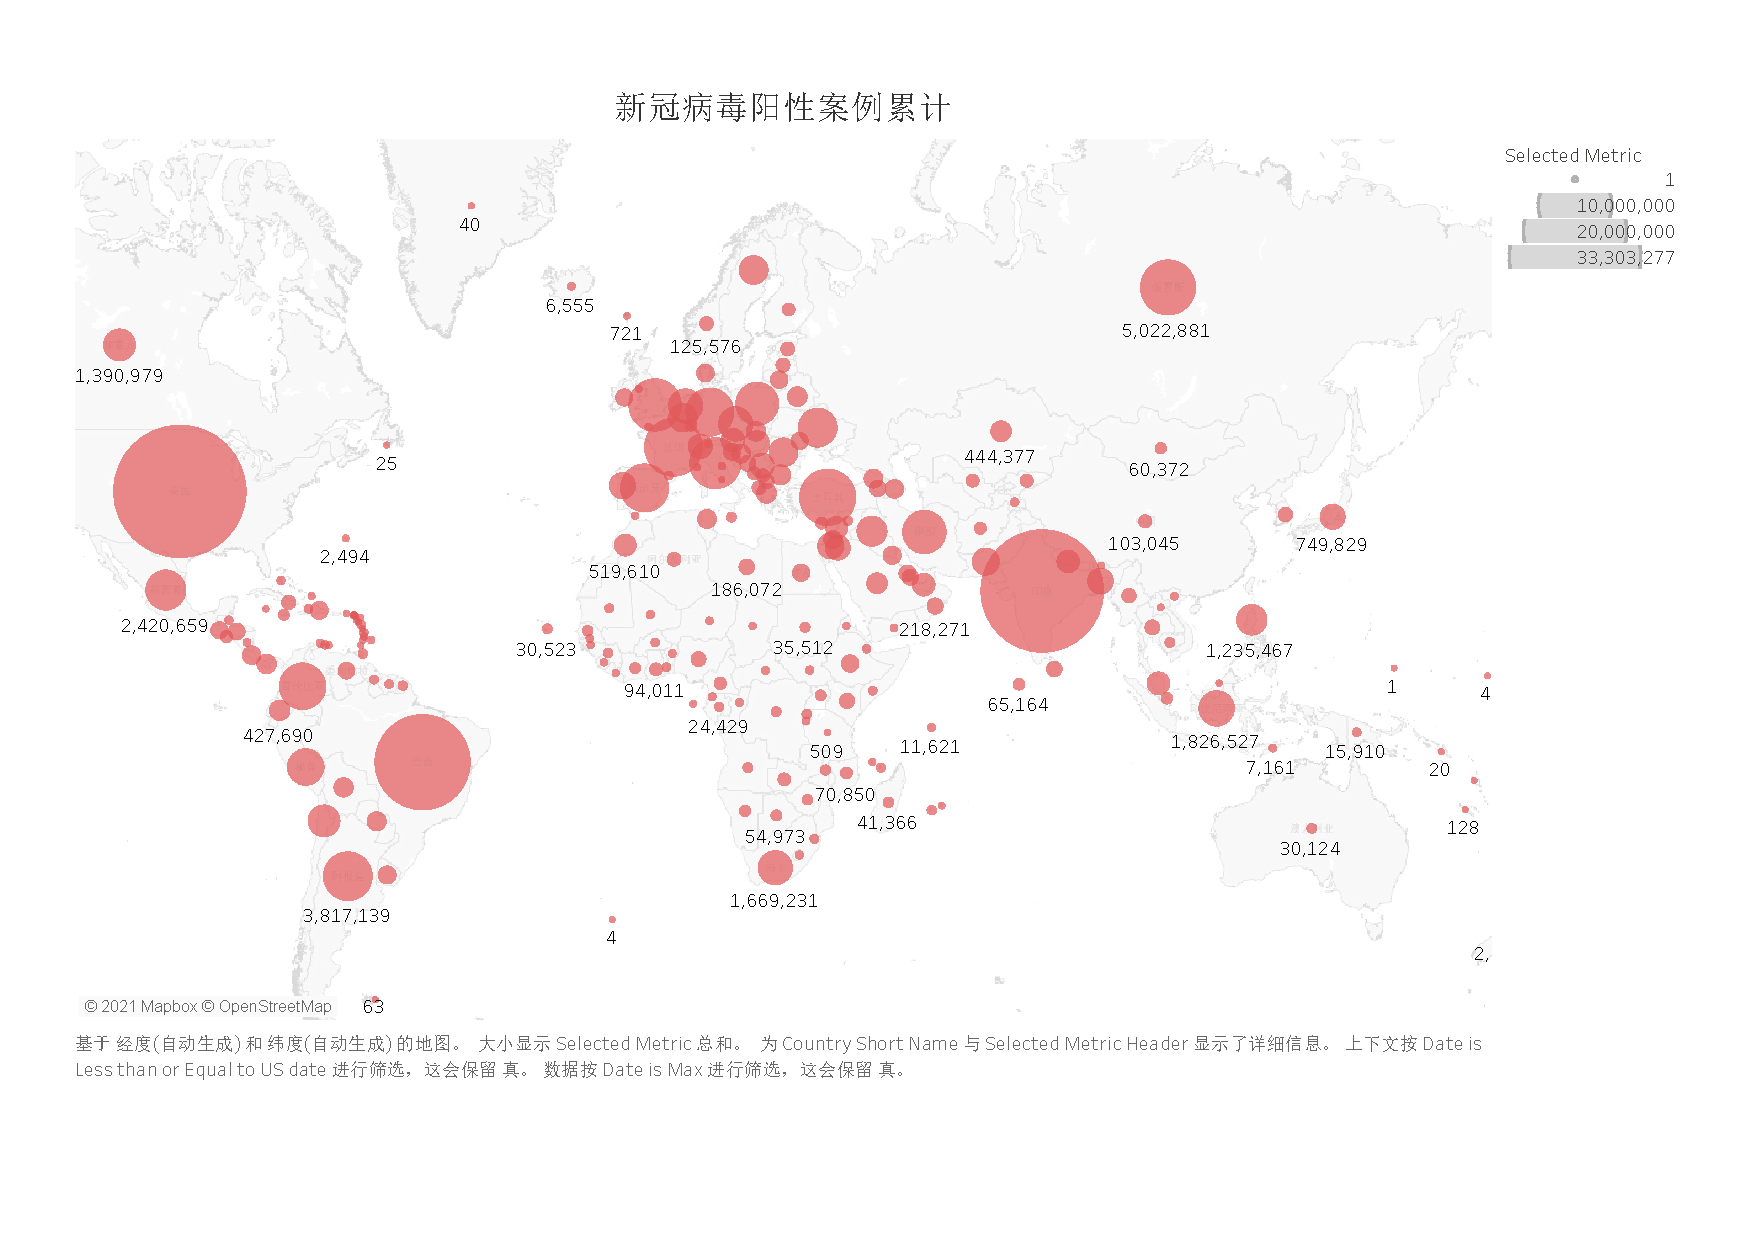
\includegraphics[height=0.7\textheight,trim=50 130 130 100,clip]{pic/Coronavirus_(COVID-19)_Cases.pdf}
			\caption{全球新冠病毒阳性案例累计}
		\end{figure}


\end{frame}
\begin{frame}{论文研究意义}
	\begin{itemize}
		\item xxxxxxx
		\item xxxxxxx
		\item xxxxxxxxxxx
	\end{itemize}

\end{frame}
\subsection{相关研究综述}
\begin{frame}{获取信息}

本文采用 Python 编写程序,爬取知网相关论文信息,共获取 $22259$ 条数据,数据包括供应商选择与评价研究相关论文的以下信息\cite{3}:

\vspace{0.5cm}

\begin{minipage}{0.4\linewidth}
\begin{itemize}
	\item 论文题目
	\item 作者
	\item 机构
	\item 发表日期
	\item 类型
\end{itemize}
\end{minipage}\hspace{1cm}
\begin{minipage}{0.3\linewidth}
\begin{itemize}
	\item 关键词
	\item 下载量
	\item 引用量
	\item 领域
	\item 基金
\end{itemize}
\end{minipage}

\vspace{0.5cm}

对获取到的数据做可视化处理。\cite{2}

\end{frame}

\begin{frame}{论文关键字词云图}
		\begin{figure}[h]
		\centering
		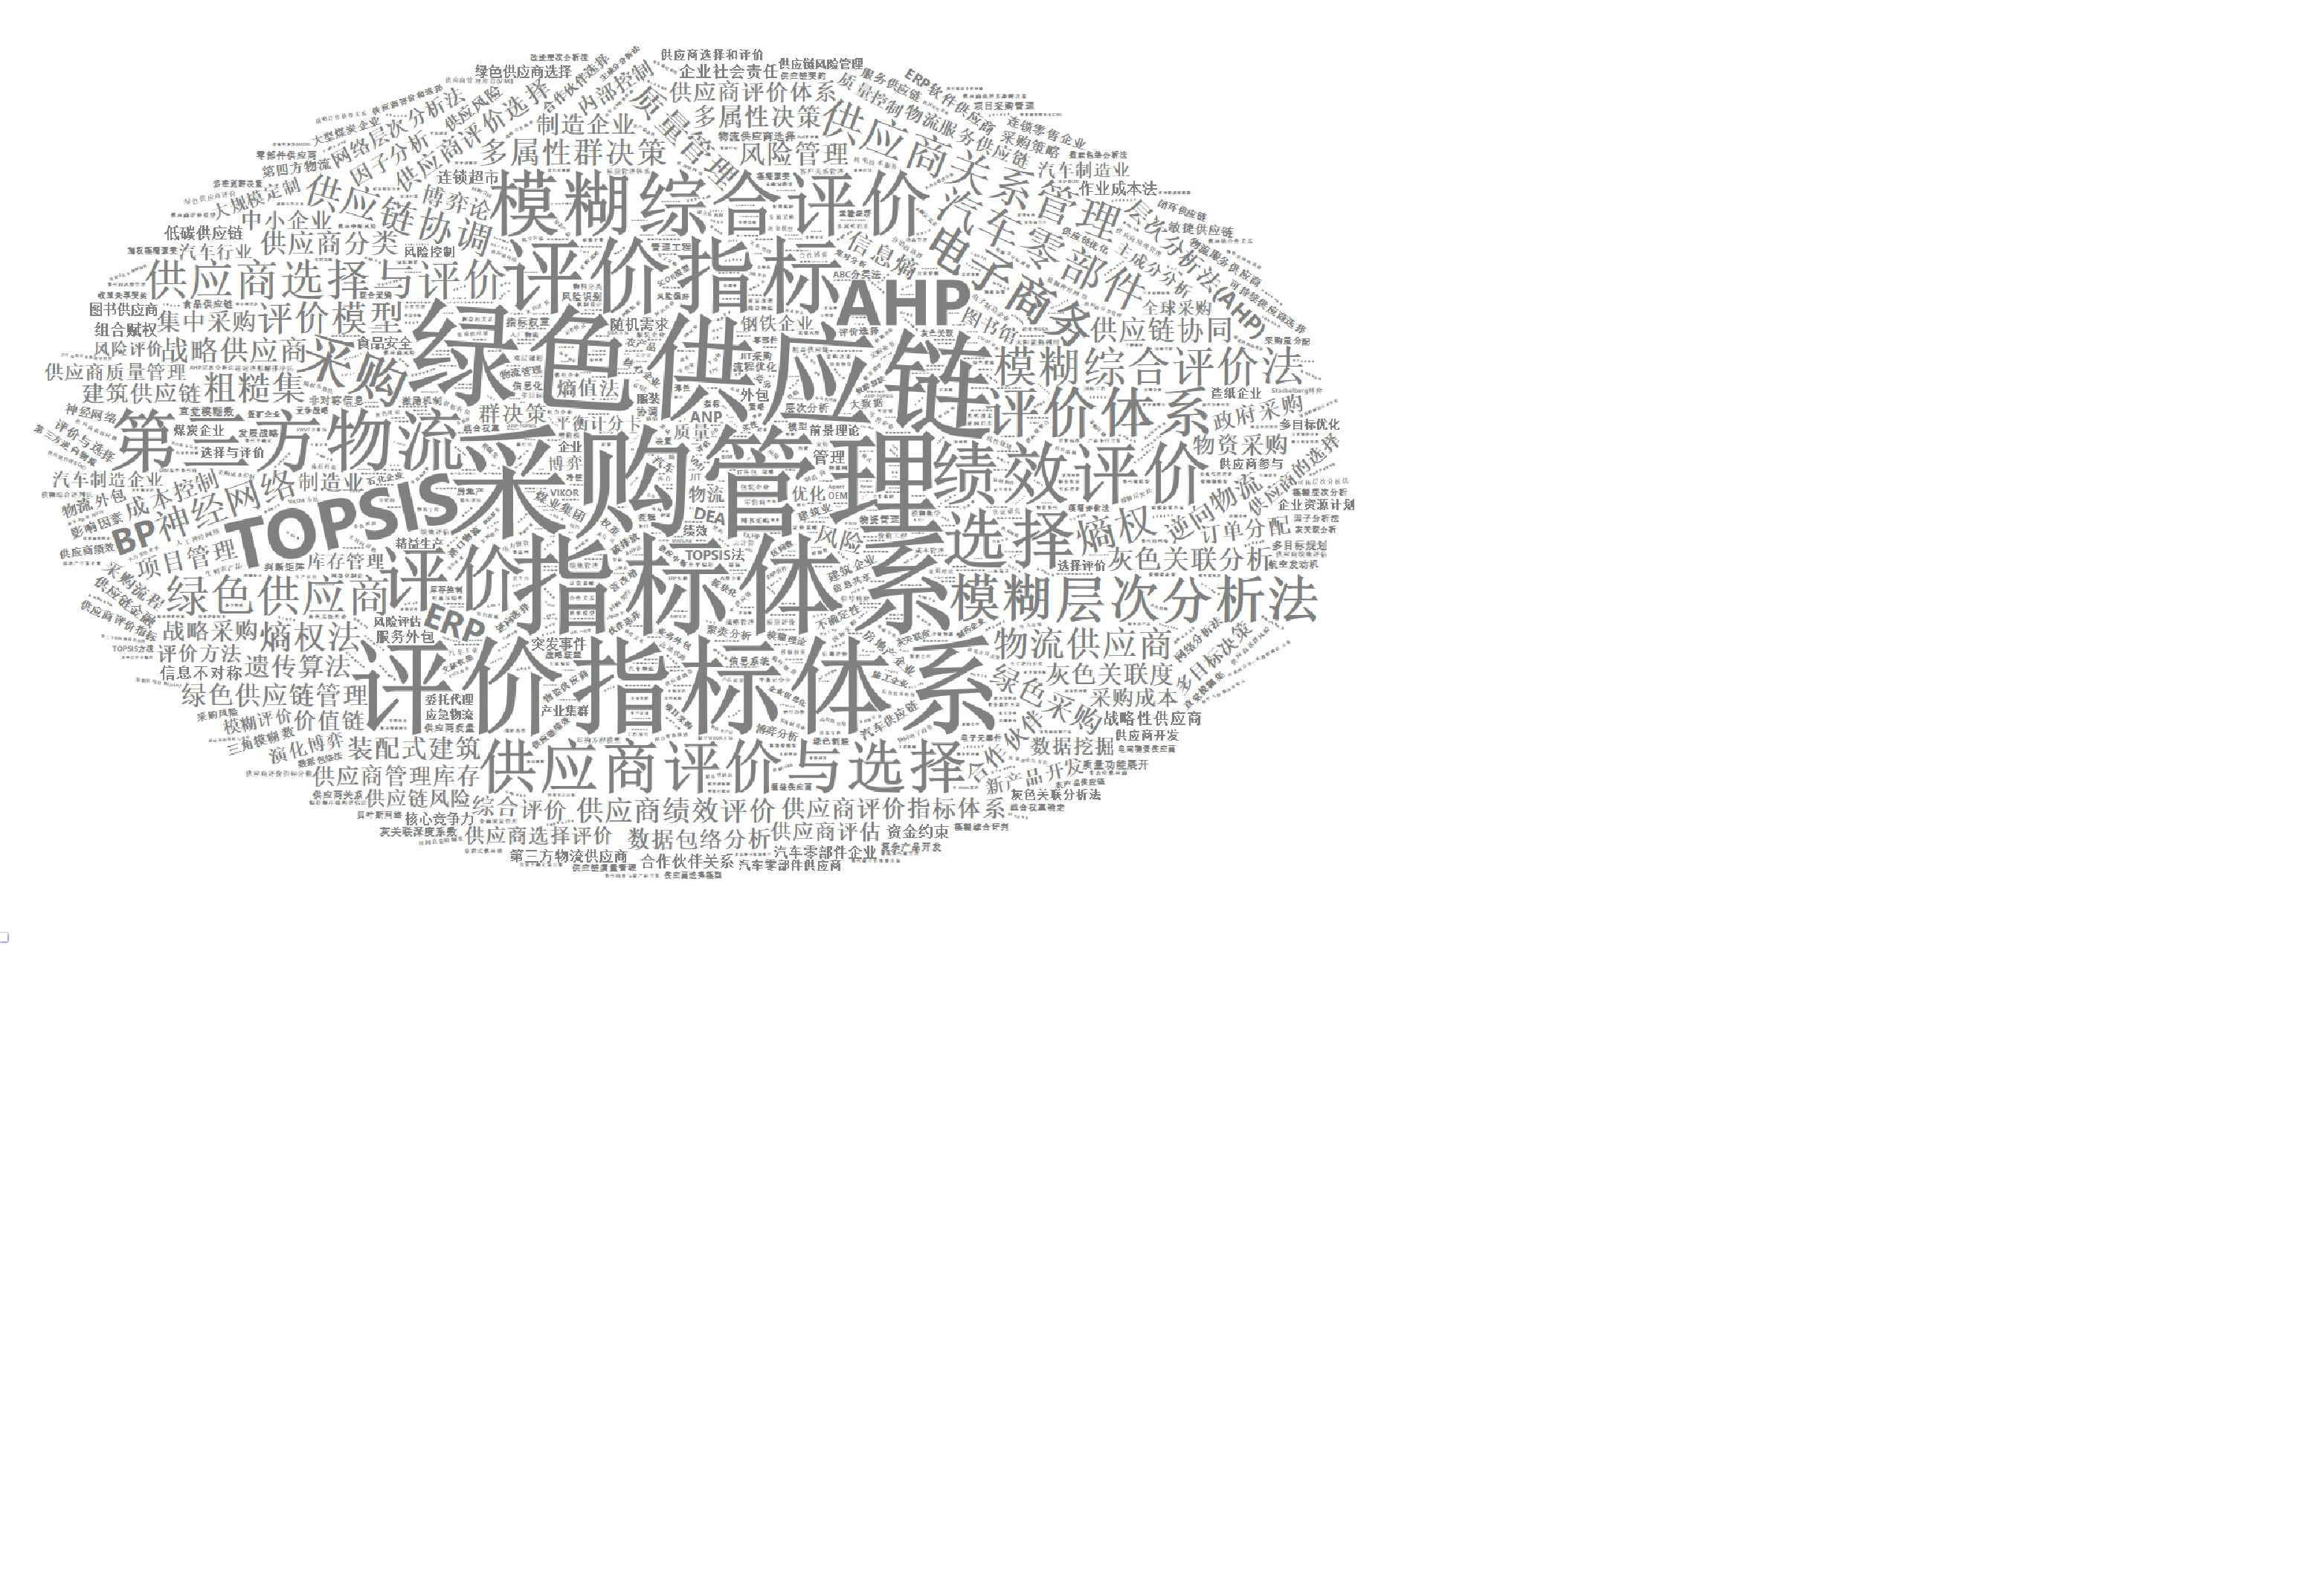
\includegraphics[height=0.76\textheight,trim=20 440 600 20,clip]{pic/wordcloud.pdf}
		\caption{论文关键字词云图}
	\end{figure}
\end{frame}

\begin{frame}{数据可视化处理}
	\vspace{-7mm}
	\begin{figure}[h]
		\centering
		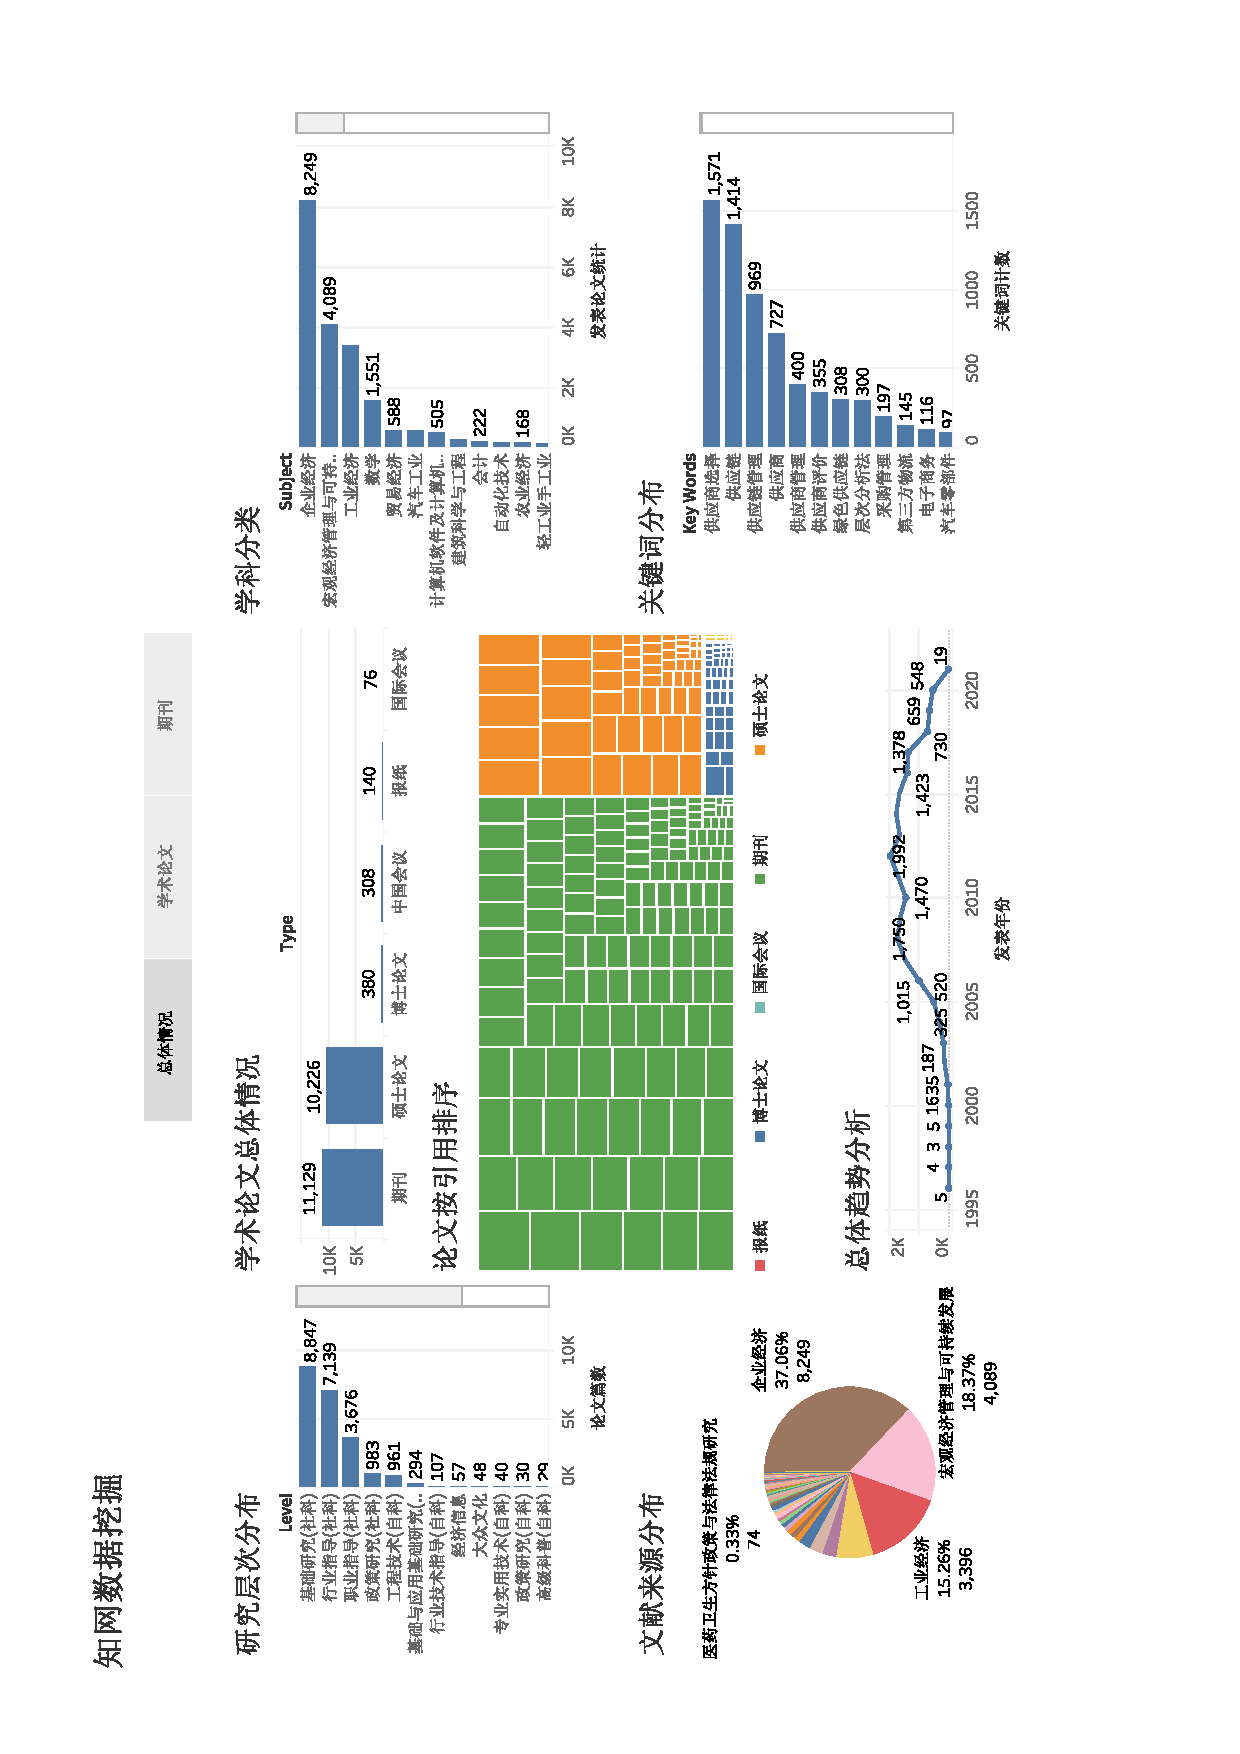
\includegraphics[height=1.4\textheight,trim=110 40 110 40,clip,angle=-90]{pic/data1.pdf}
		\caption{按多种查询方法得出的分析总体情况}
	\end{figure}
\end{frame}

\begin{frame}{数据可视化处理}
	\vspace{-7mm}
	\begin{figure}[h]
		\centering
		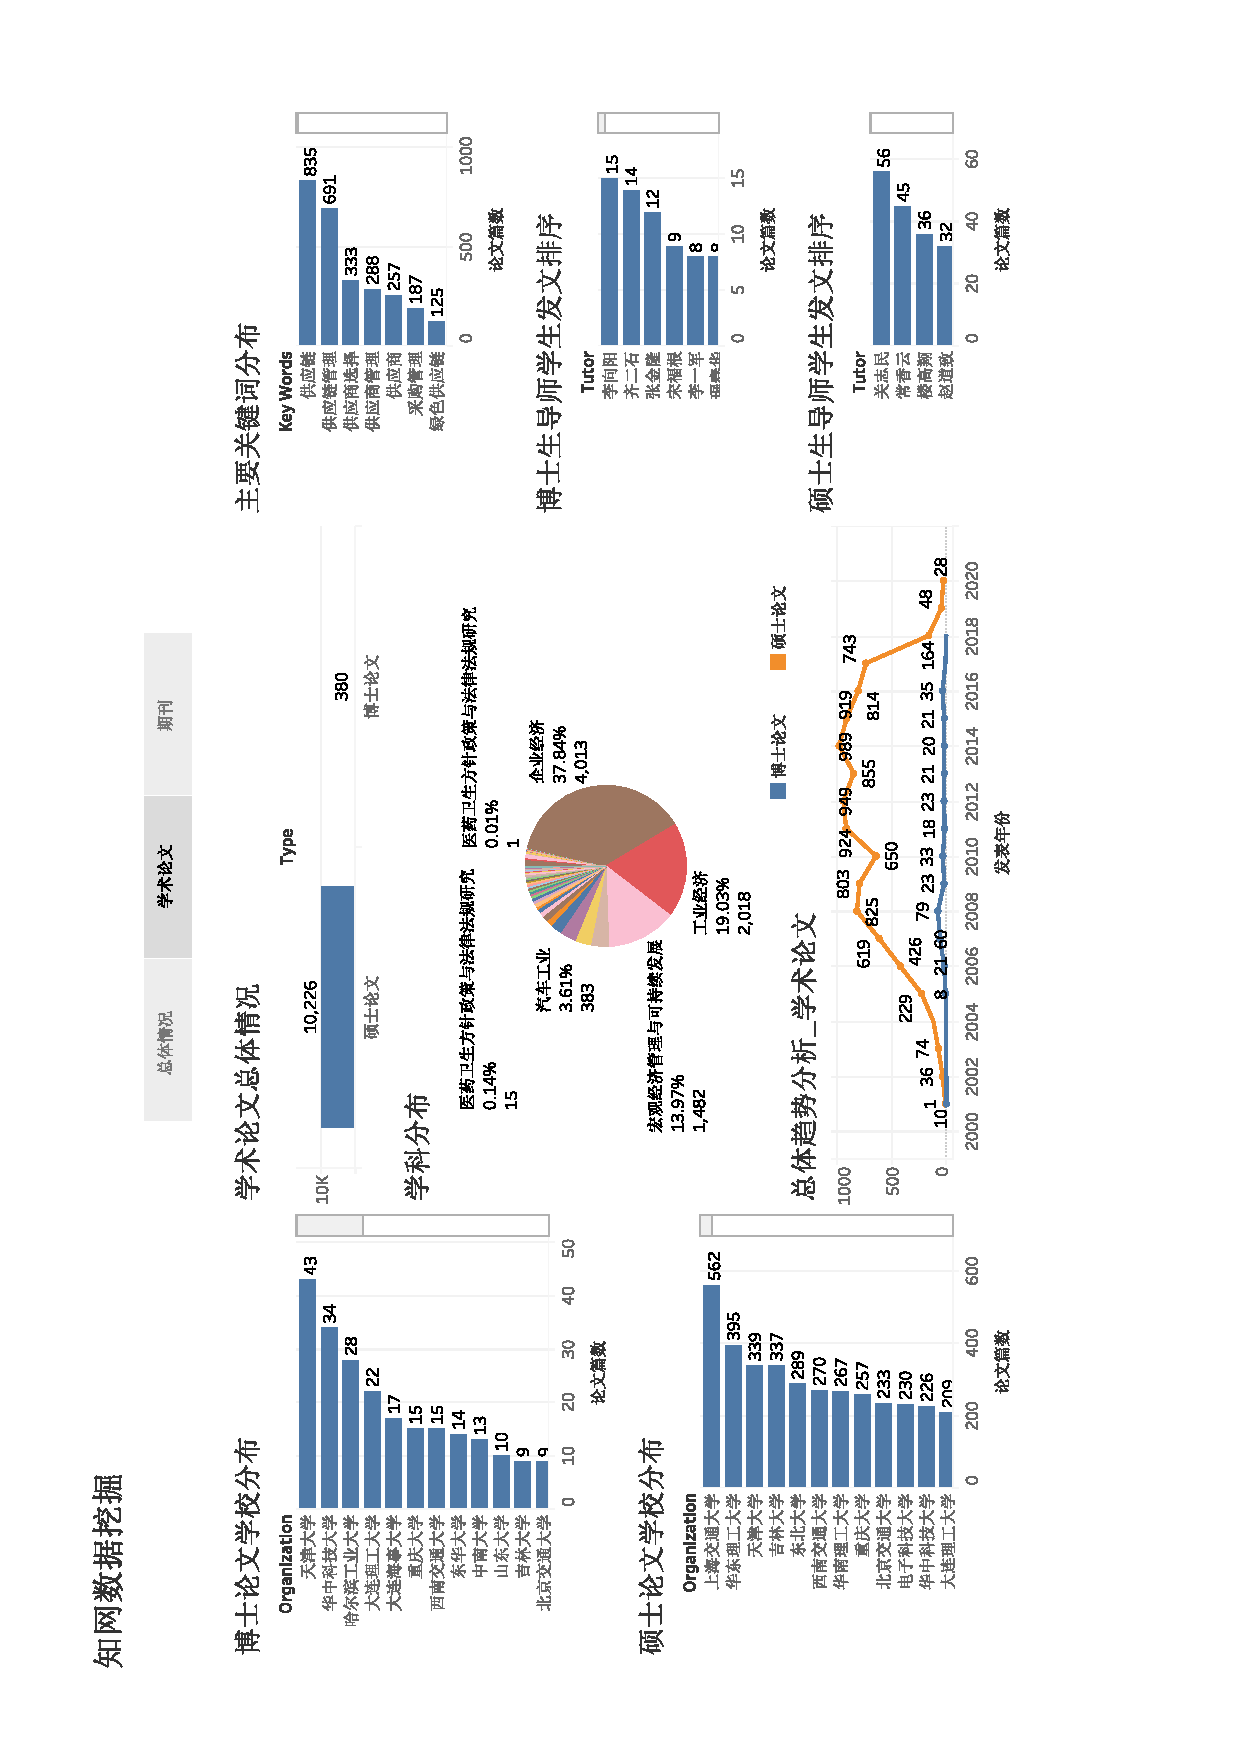
\includegraphics[height=1.4\textheight,trim=110 40 110 40,clip,angle=-90]{pic/data2.pdf}
		\caption{学位论文查询结果统计}
	\end{figure}
\end{frame}

\begin{frame}{数据可视化处理}
	\vspace{-7mm}
	\begin{figure}[h]
		\centering
		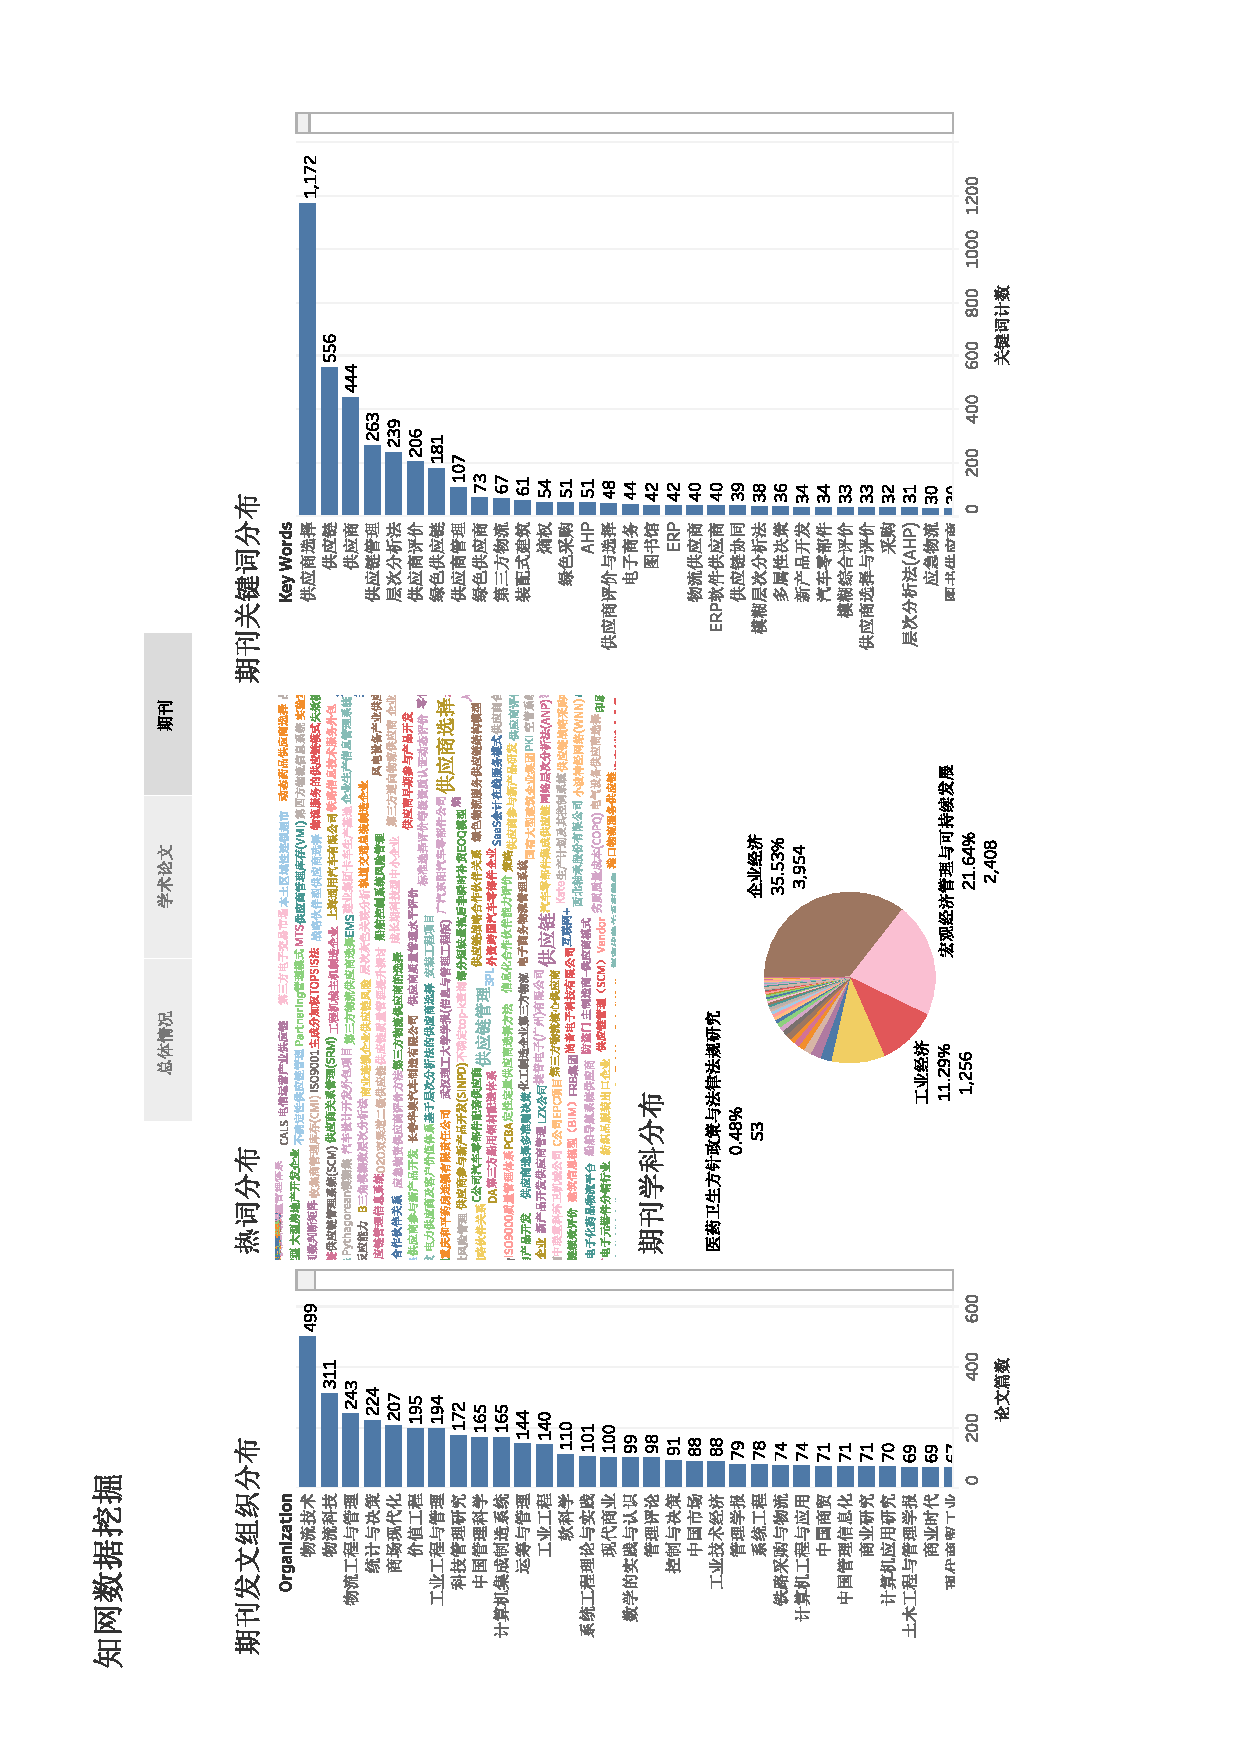
\includegraphics[height=1.4\textheight,trim=110 40 110 40,clip,angle=-90]{pic/data3.pdf}
		\caption{期刊论文查询结果统计}
	\end{figure}
\end{frame}

\subsection{研究思路}

\begin{frame}{研究思路}
	\begin{minipage}{0.2\linewidth}
	\vspace{-3mm}
\begin{figure}[h]
	\centering
	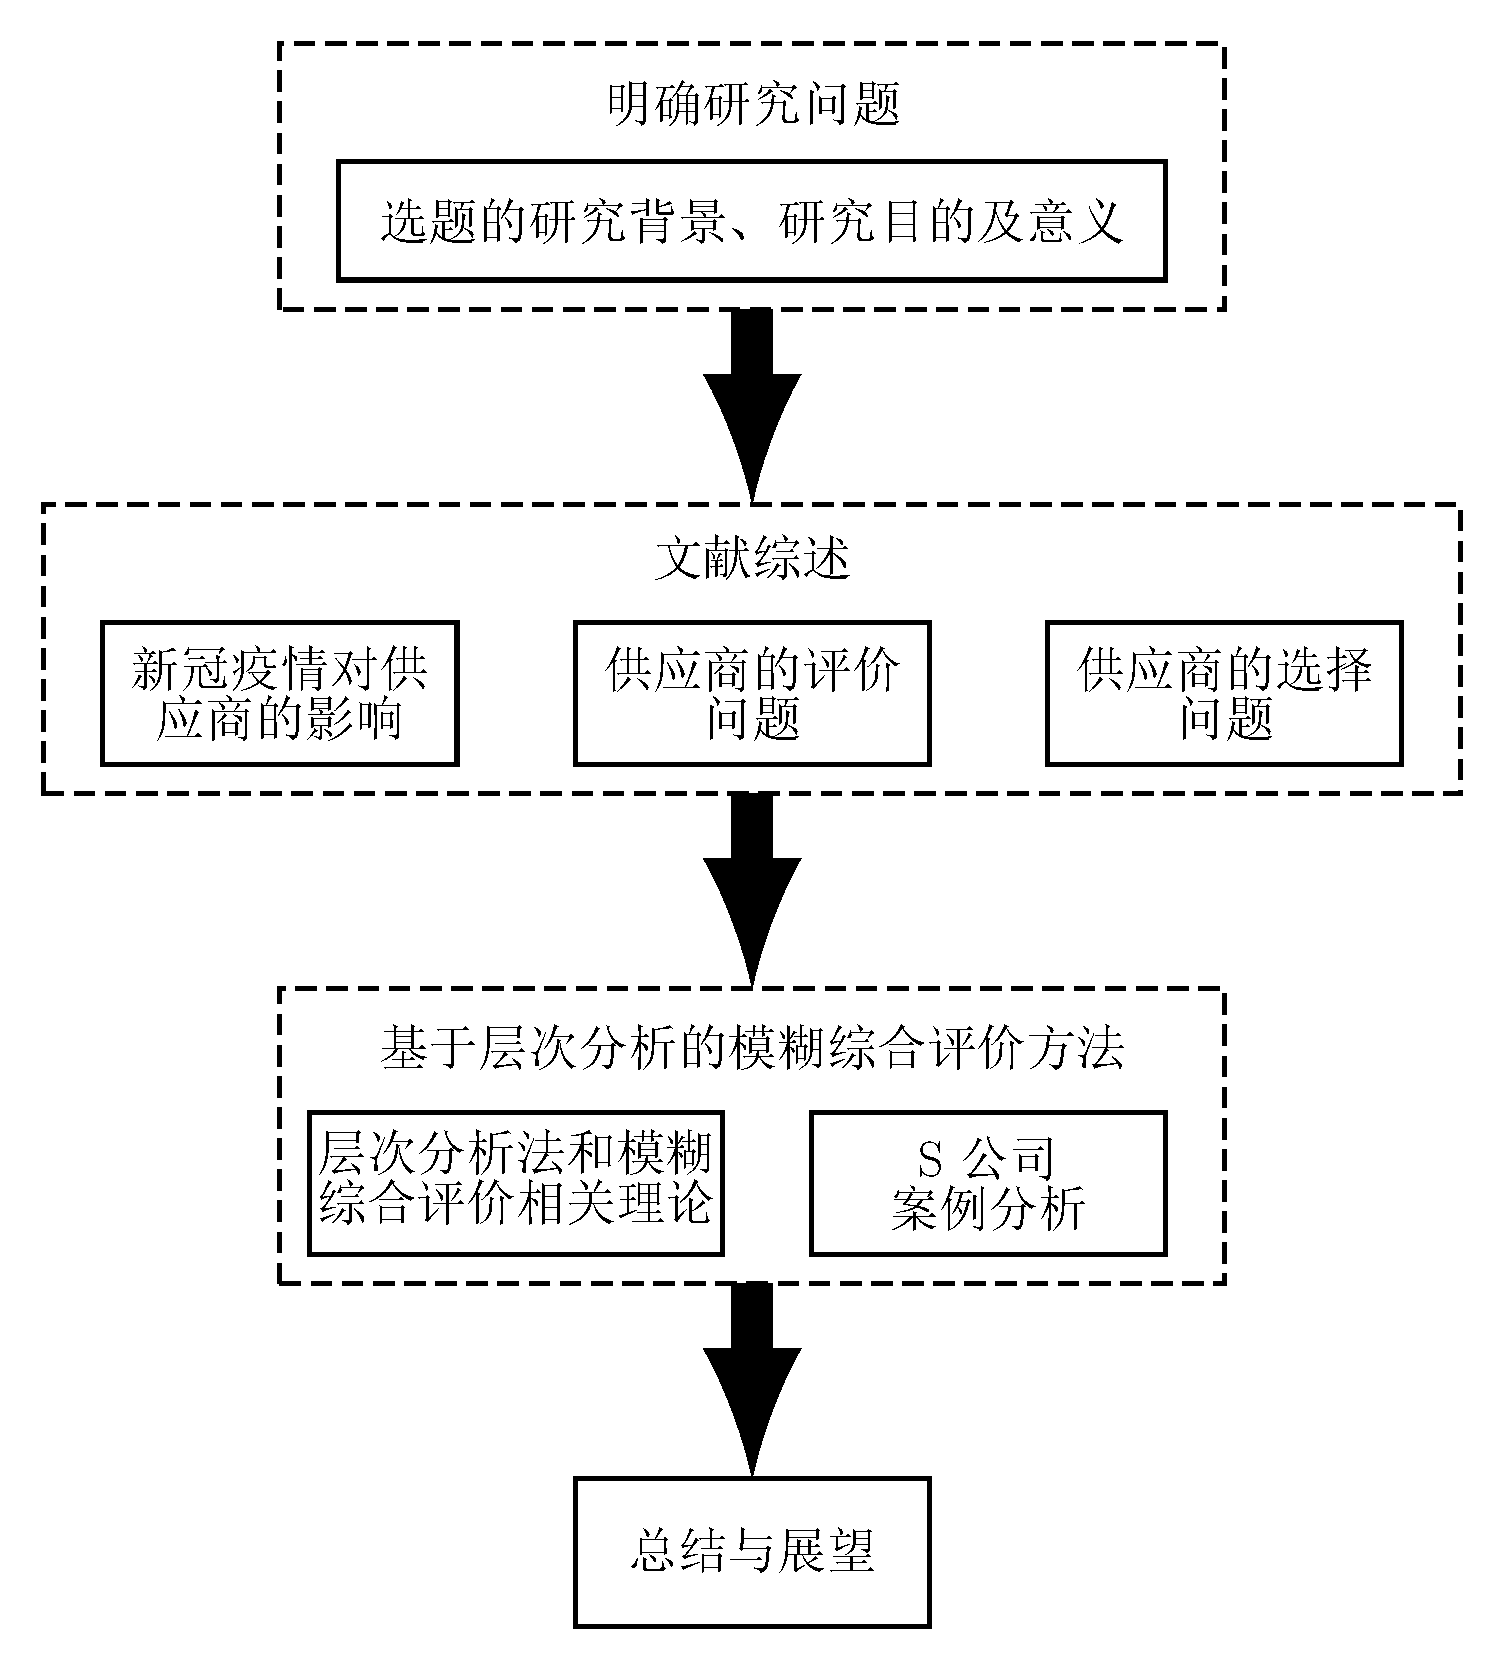
\includegraphics[height=0.95\textheight,trim=0 0 0 0,clip]{pic/研究思路.pdf}
\end{figure}
	\end{minipage}\hspace{4.3cm}
	\begin{minipage}{0.38\linewidth}
		\vspace{-3mm}
		\footnotesize{
		\begin{itemize}
			\item 绪论
				\begin{itemize}
				\scriptsize
				\item 论文研究背景及意义 
				\item 相关研究综述
				\item 本文主要内容
			\end{itemize}
			\item 供应商质量评价指标体系
				\begin{itemize}
				\scriptsize
				\item 相关理论
				\item 供应商综合评价指标体系
				\item 本章小结
			\end{itemize}
			\item 基于层次分析的模糊综合评价方法
				\begin{itemize}
				\scriptsize
				\item 层次分析法概述
				\item 基于模糊综合评价方法选择供应商 
			\end{itemize}
			\item 案例分析
			\item 总结与展望
		\end{itemize}}
	\end{minipage}
\end{frame}

\section{供应商质量评价指标体系}
\subsection{相关理论}
\begin{frame}{相关理论}
	\vspace{-3mm}
	\begin{figure}[h]
		\centering
		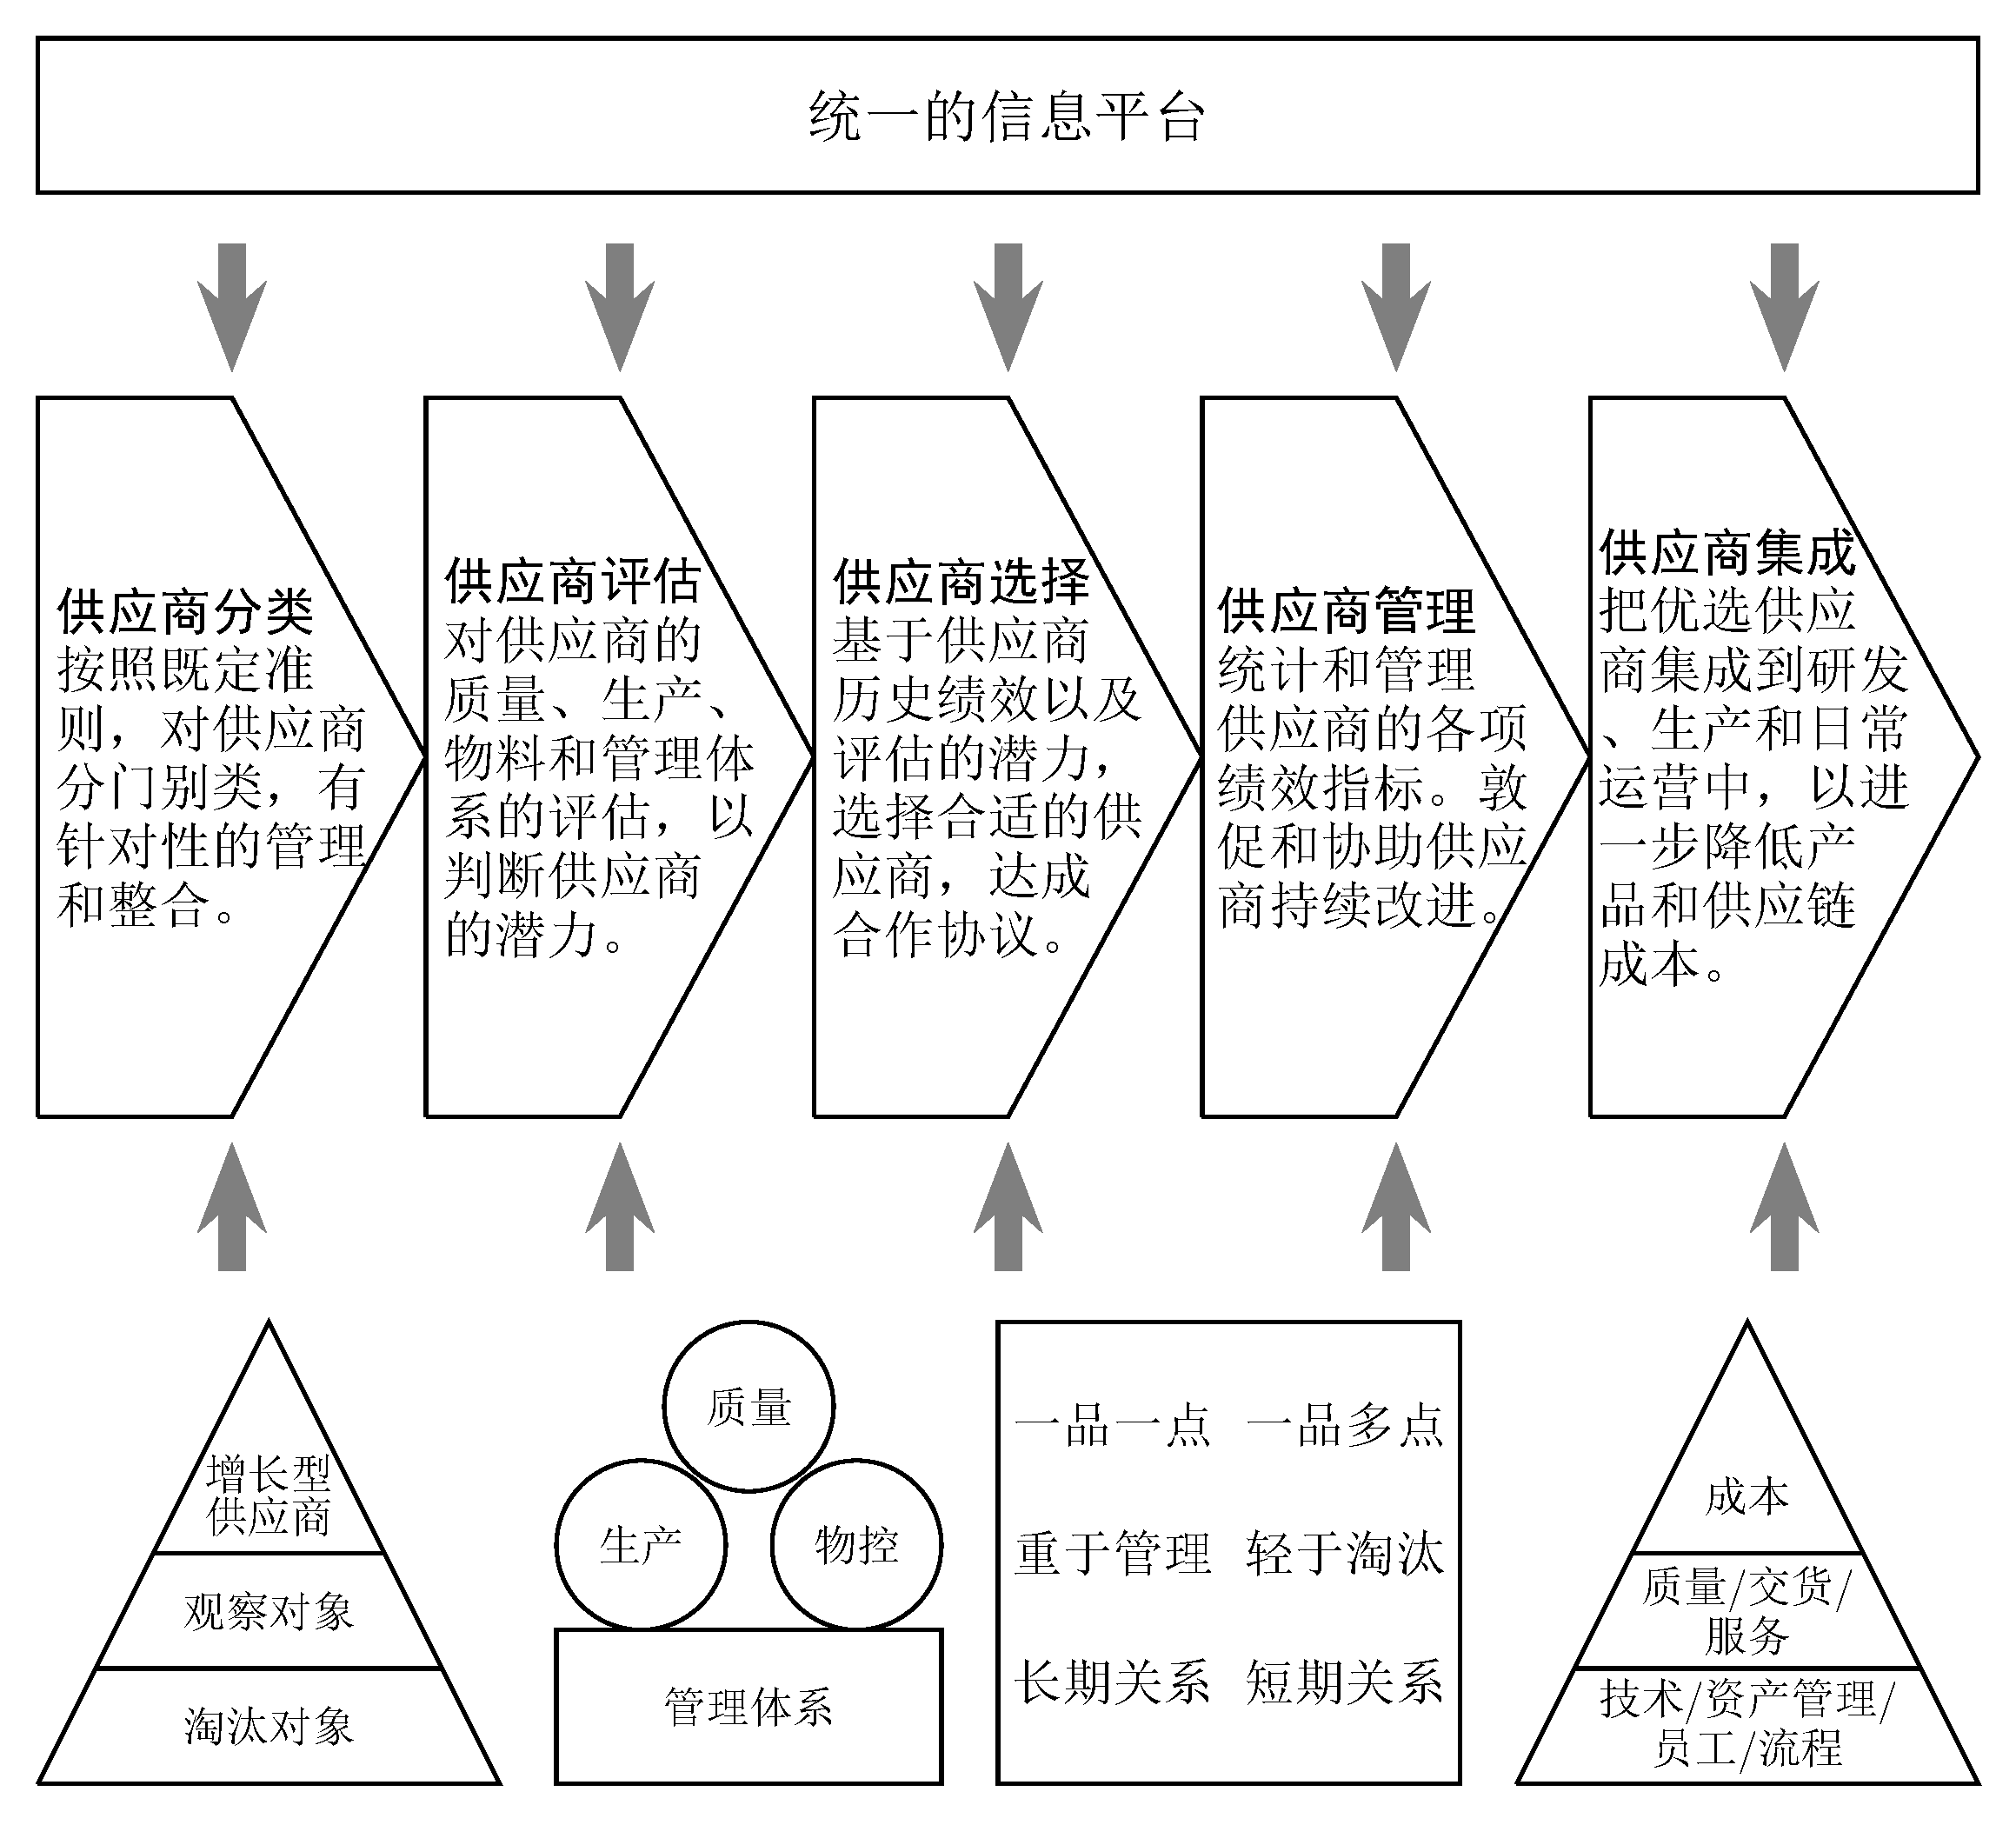
\includegraphics[height=0.9\textheight,trim=0 20 0 0,clip]{pic/供应商管理的流程.pdf}
	\end{figure}
\end{frame}

\subsection{供应商综合评价指标体系}
\begin{frame}
	
	\begin{block}{对传统供应链短板的分析}
	\begin{itemize}
		\item xxxxxxx
		\item xxxxxxx
	\end{itemize}
\end{block}

\begin{block}{后新冠疫情时代供应商评价指标的考量}
		\begin{itemize}
		\item xxxxxxxxxxxxxxxxxxxxx
		\item xxxxxxxxxxxxxxxxxx
		\item xxxxxxxxxxxx
	\end{itemize}
	\end{block}

\end{frame}

\begin{frame}{供应商综合评价指标体系的构建}
\vspace{-3mm}
\renewcommand{\arraystretch}{1.5}	
\begin{table}[h]  
	\scriptsize
	\centering
	\caption{供应商综合评价指标}   
	\label{体系}
	\begin{tabular}{p{2cm}lp{2cm}l}    
		\toprule    
		一级指标&二级指标&一级指标&二级指标\\
		\midrule   
		\multirow{4}{3cm}{产品质量}&产品合格率&\multirow{4}{3cm}{供货能力}&数字化交付能力\\
		&返工率&&品种满足率\\
		&退货率 &&产能利用率\\
		&过程能力 &&库存周转率\\
		\cline{1-4}  
		\multirow{4}{3cm}{财务状况}& 资产负债率&\multirow{4}{3cm}{技术水平}&$R\& D$投入比\\
		&成本降低率&&ISO认证率 \\
		&报价能力&&专业人才占比\\
		&流动资产周转率&&产品标准化程度\\
		\cline{1-4}
		\multirow{4}{3cm}{管理水平}  &信息化水平&\multirow{4}{3cm}{合作能力}  &市场占有率\\
		&员工离职率&&员工离职率\\\
		&抗风险能力&&抗风险能力 \\
		\bottomrule   
	\end{tabular}  
\end{table}

\end{frame}

\section{xxxxxxxxxxxxxxxxxx}

\subsection{xxxxxxxxxxxxxx}

\begin{frame}{xxxxxxxxxxxxxxxxx}
		\begin{figure}[h]
	\centering
	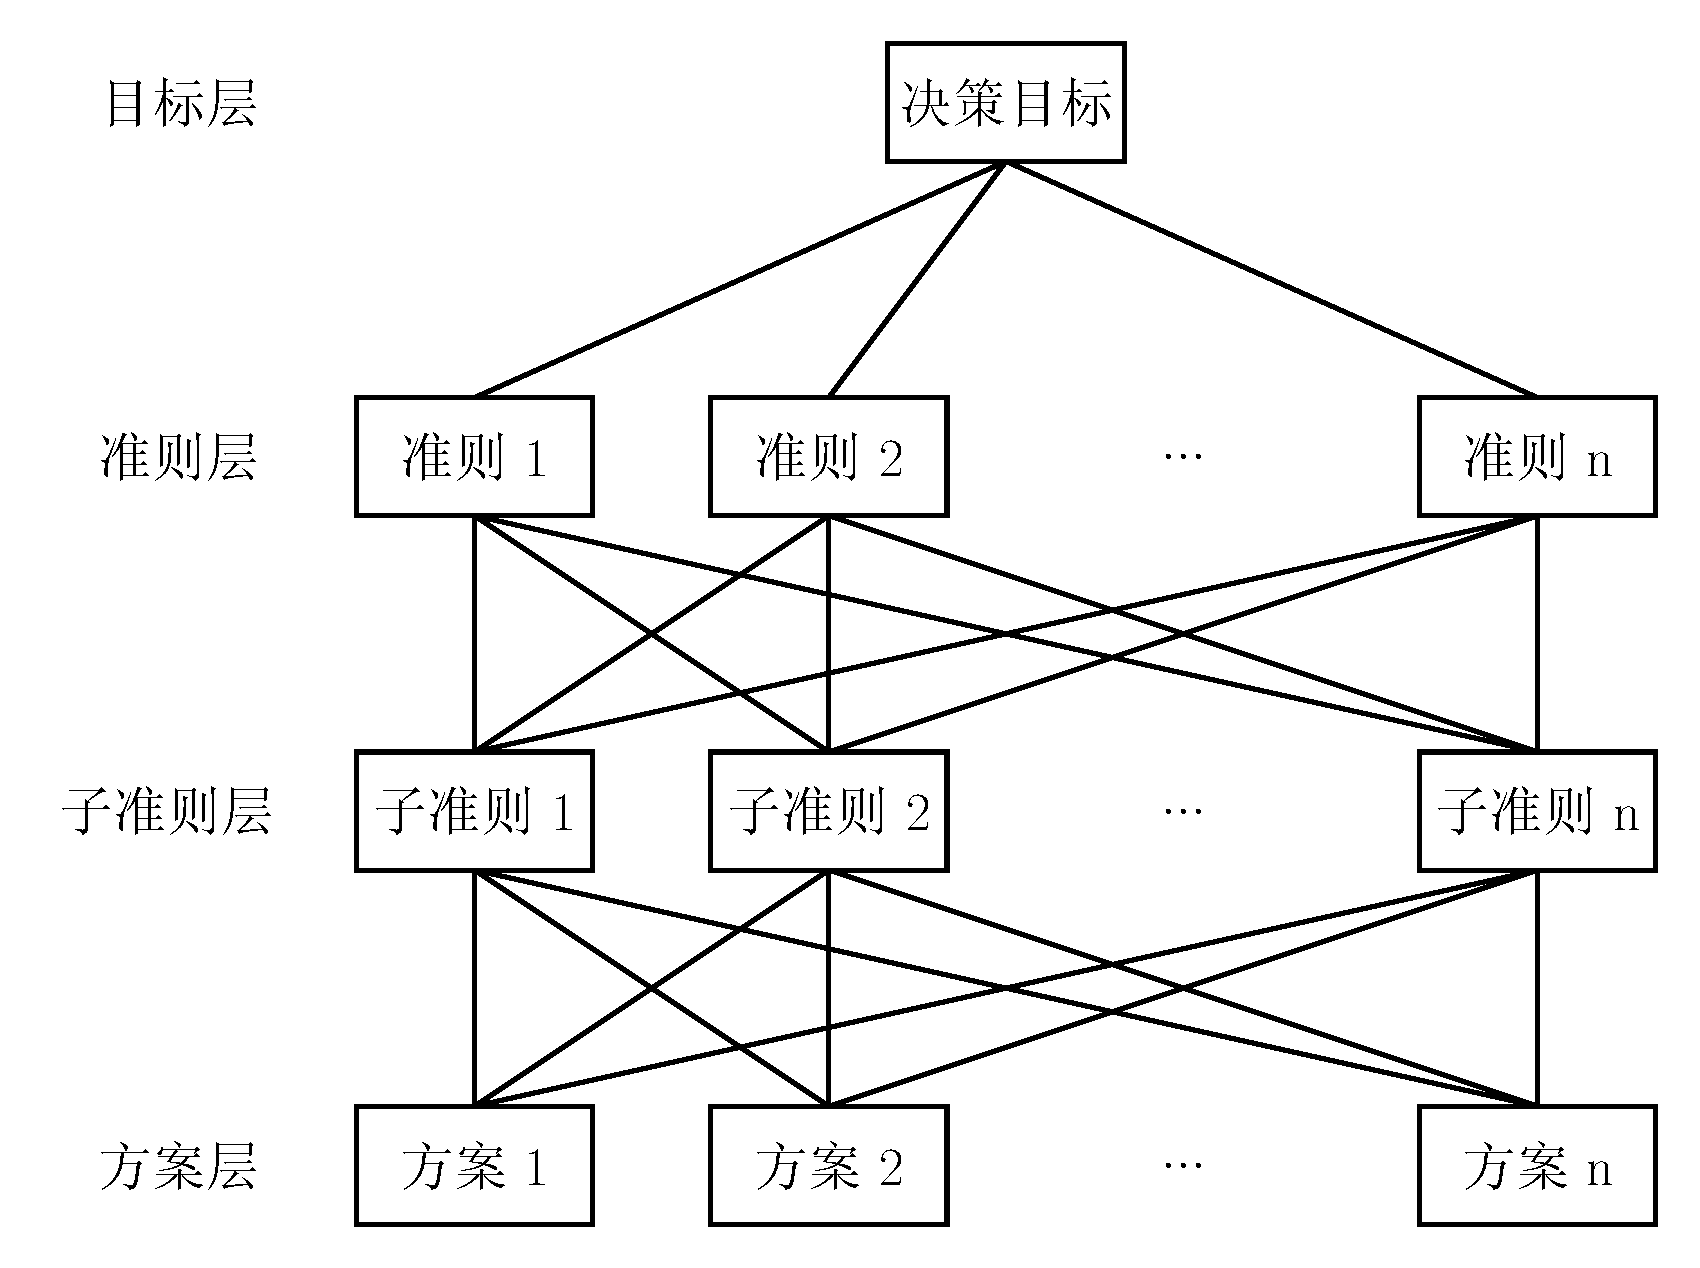
\includegraphics[height=0.76\textheight,trim=0 0 0 0,clip]{pic/递进层次结构示意图.pdf}
	\caption{递进层次结构示意图}
\end{figure}
\end{frame}

\subsection{xxxxxxxxxxxxxx}

\begin{frame}{xxxxxxxxxxxxxx}
	\begin{block}{概述}
	xxxxxxxxxxxxxxxxxxxxxxxxxxxxxxxxxxxxxxxxxxxxxx
	
	xxxxxxxxxxxxxxxxxxxxxxxxxxxxxxxx
	\end{block}
\begin{block}{基本步骤}
\begin{itemize}
	\item xxxxxxxxxxxx
	\item xxxxxxxxxxxx
	\item xxxxxxxxxxxx
\end{itemize}
\end{block}


\end{frame}

\section{案例分析}
\subsection{案例背景}
\begin{frame}{案例背景}

\qquad xxxxxxxxxxxxxxxxxxxxxxxxxxxxxxxxx
\vspace{5mm}
\begin{itemize}
	\item xxxxxx
	\item xxxxxx
	\item xxxxxx
\end{itemize}

\end{frame}

\subsection{xxxxxxxxxxxxxxxxx}
	\begin{frame}{xxxxxxxxxxxxxxx}
		\vspace{-7mm}
		\begin{figure}[h]
	\centering
	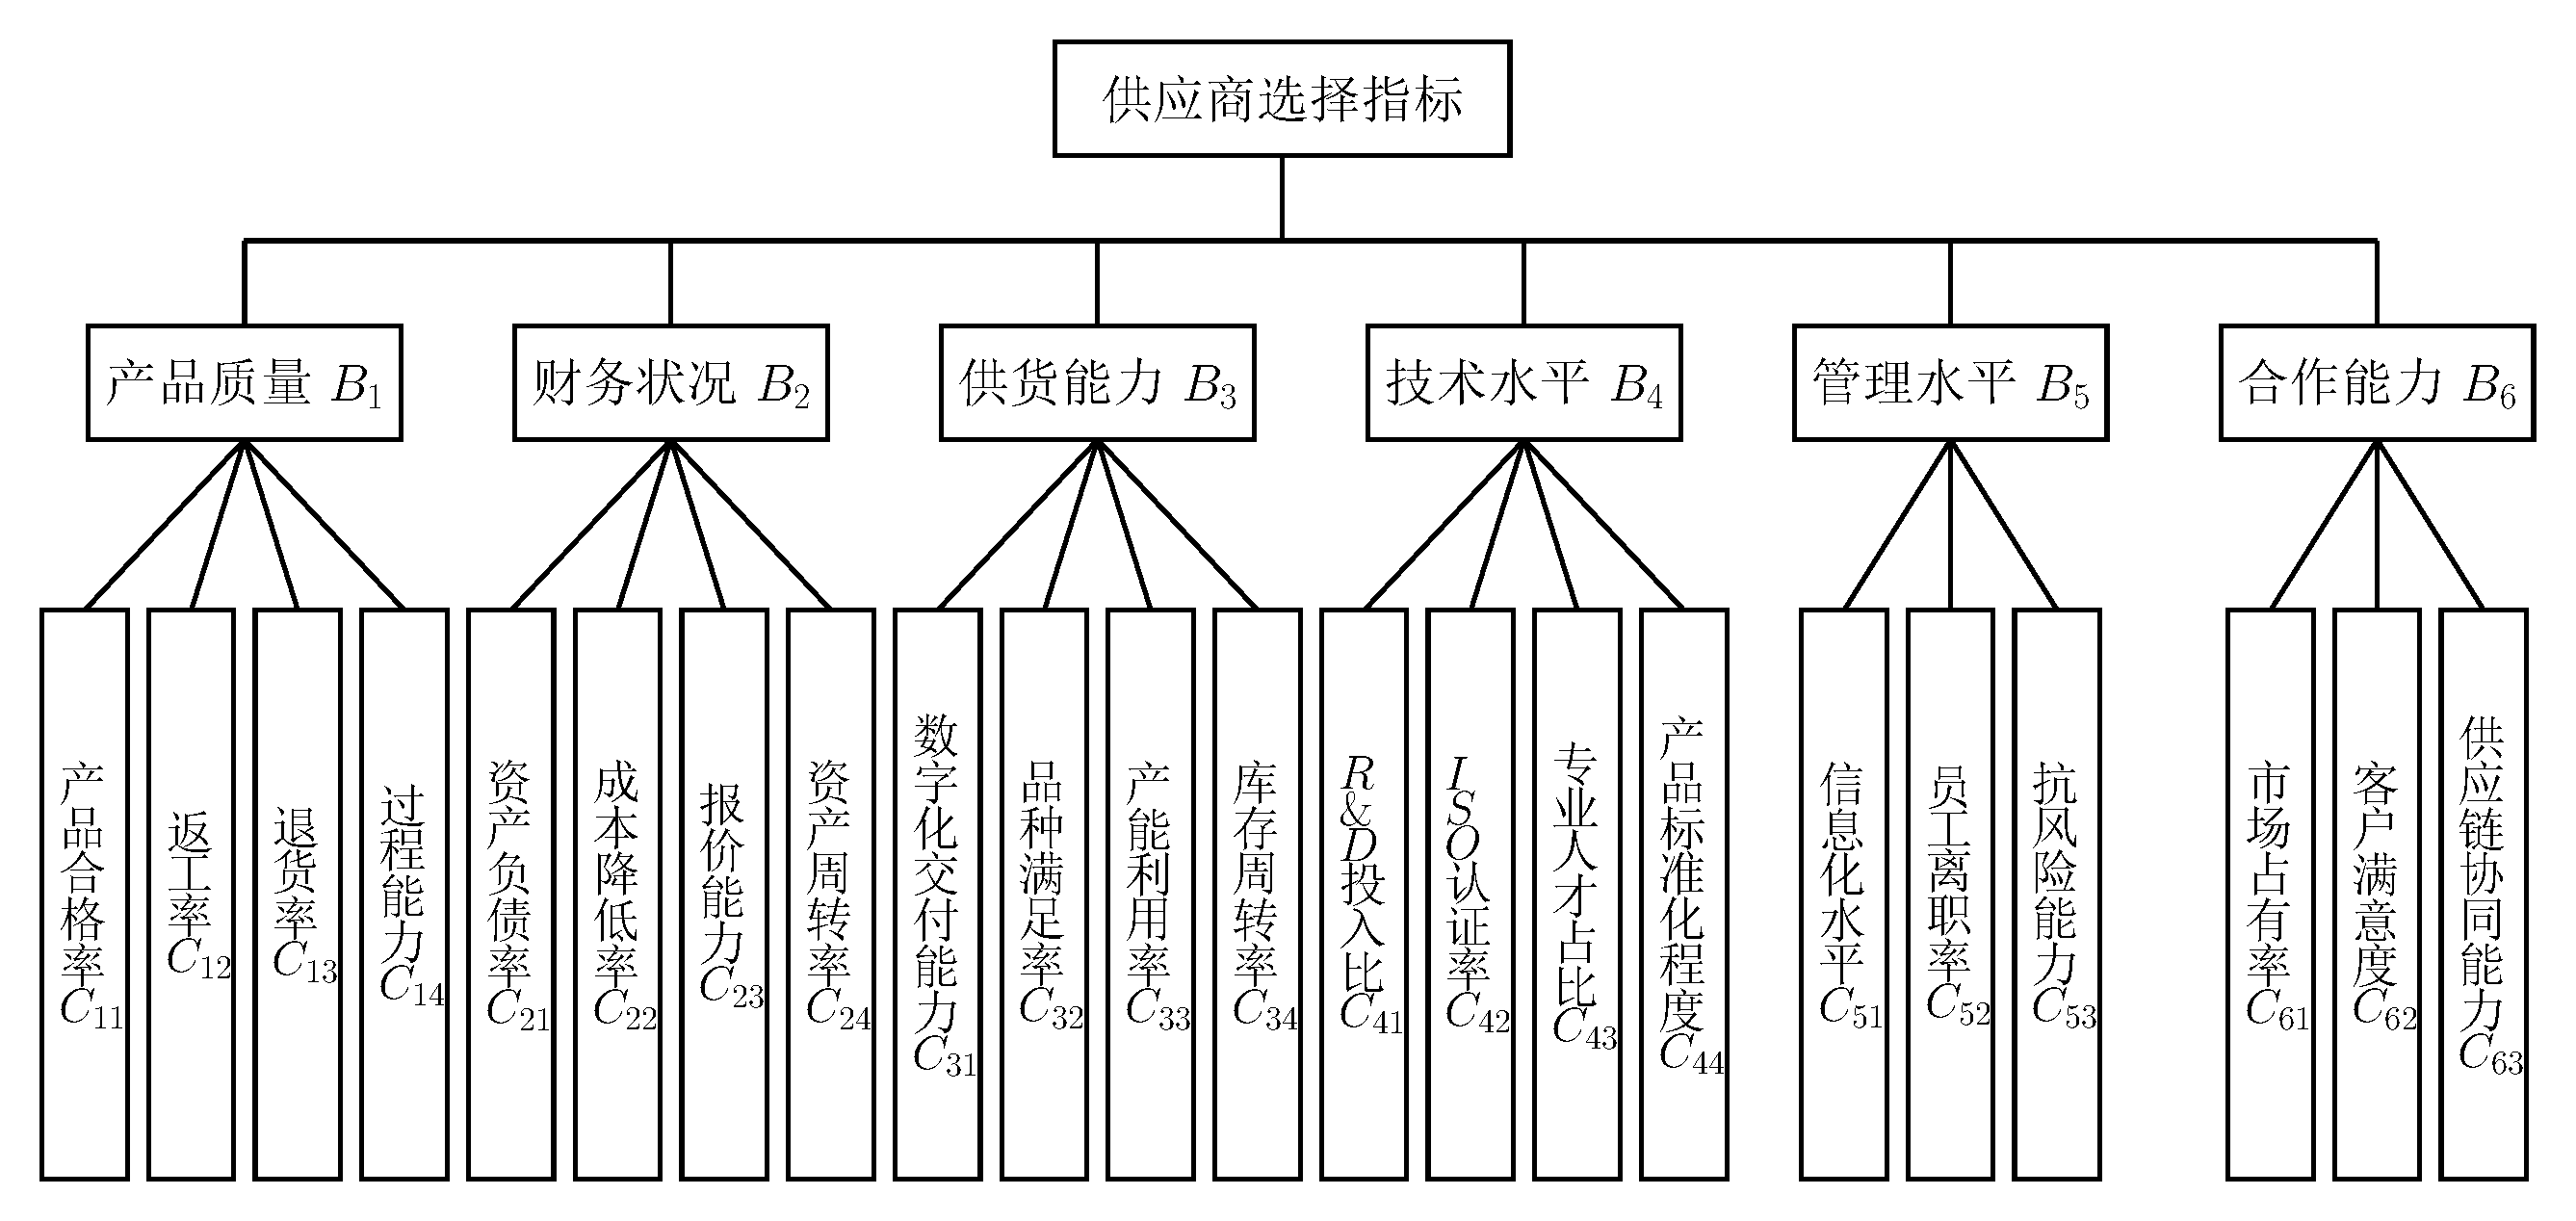
\includegraphics[height=0.65\textheight,trim=10 0 0 0,clip]{pic/递进层次结构示意图_2.pdf}
	\caption{供应商评价指标的递阶层次结构图}
	\label{递进层次结构示意图_2}
\end{figure}
	\end{frame}

\begin{frame}{xxxxxxxxxxxxxx}

xxxxxxxxxxxxxxxxxxxxxxxxxxxxxxxxxxxxxxxxxxxxxxxxxxxxxxxxxxxxxxxxxxxxxxxxxxxxxxxxxxxxxxxxxxxxxxxxxxxxxxxxxxxxxxxxxxxxxxxxxxxxxxxxxxxxxxxxxxxxxxxxxxxxxxxxxxxxxxxxxxxxxxxxxxxxxxxxxxxxxxxxxxxxxxxxxxxxxxxxxxxxxxxxxxxxxxxxxxxxxxxxxxxxxxxxxxxxxxxxxxxxxxxxxxxxxxxxxxxxxxxxxxxxxxxxxxxxxxxxxxxxxxxxxxxxxxxxxxxxxxxxxxxxxxxxxxxxxxxxxxxxxxxxxxxxxxxxxxxxxxxxxxxxxxxxxxxxxxxxxxxx
\vspace{-5mm}
\begin{equation}
		 \scriptsize
	A_i=\left[ \begin{matrix}
		1 & 4&2 &5 &6& 3   \\
		\dfrac{1}{4} & 1&\dfrac{1}{3} &2 &3&\dfrac{1}{2}  \\
		\dfrac{1}{2} & 3 &1 &3 &4 &2\\
		\dfrac{1}{5} & \dfrac{1}{2} &\dfrac{1}{3} &1 &2 &\dfrac{1}{2}\\
		\dfrac{1}{6} & \dfrac{1}{3} &\dfrac{1}{4} &\dfrac{1}{2} &1 &\dfrac{1}{5}\\
		\dfrac{1}{3} & 2 &\dfrac{1}{2} &2 &5 &1\\
	\end{matrix} \right] 
\end{equation}
\end{frame}

\begin{frame}{xxxxxxxxxxxxxxx}
	
xxxxxxxxxxxxxxxxxxxxxxxxxxxxxxxxxxxxxxxxxxxxxxxxxxxxxxxxxxxxxxxxxxxxxxxxxxxxxxxxxxxxxxxxxxxxxxxxxxxxxxxxxxxxxxxxxxxxxxxxxxxxxxxxxxxxxxxxxxxxxxxxxxxxxxxxxxxxxxxxxxxxxxxxxxxxxxxxxxxxxxxxxxxxxxxxxxxxxxxxxxxxxxxxxxxxxxxxxxxxxxxxxxxxxxxxxxxxxxxxxxxxxxxxxxxxxxxxxxxxxxxxxxx

	\begin{minipage}{0.45\linewidth}
				 \scriptsize
\begin{equation}
	\label{a21}
	A_{21}=\left[ \begin{matrix}
		1&2&4&5\\
		\dfrac{1}{2}&1&3&4\\
		\dfrac{1}{4}&\dfrac{1}{3}&1&3\\
		\dfrac{1}{5}&\dfrac{1}{4}&\dfrac{1}{3}&1\\
	\end{matrix} \right] 
\end{equation}
	\end{minipage}
\begin{minipage}{0.45\linewidth}
			\scriptsize
\begin{equation}
	\label{a22}
	A_{22}=\left[ \begin{matrix}
		1&\dfrac{1}{3}&\dfrac{1}{5}&\dfrac{1}{2}\\
		3&1&\dfrac{1}{3}&2\\
		5&3&1&4\\
		2&\dfrac{1}{2}&\dfrac{1}{4}&1\\
	\end{matrix} \right] 
\end{equation}	
	\end{minipage}

\begin{minipage}{0.45\linewidth}
		 \scriptsize
\begin{equation}
	\label{a23}
	A_{23}=\left[ \begin{matrix}
		1&5&2&3\\
		\dfrac{1}{5}&1&\dfrac{1}{7}&\dfrac{1}{4}\\
		\dfrac{1}{2}&7&1&2\\
		\dfrac{1}{3}&4&\dfrac{1}{2}&1\\
	\end{matrix} \right] 
\end{equation}
	\end{minipage}
\begin{minipage}{0.45\linewidth}
		\scriptsize
\begin{equation}
	\label{a24}
	A_{24}=\left[ \begin{matrix}
		1&\dfrac{1}{4}&2&\dfrac{1}{2}\\
		4&1&6&3\\
		\dfrac{1}{2}&\dfrac{1}{6}&1&\dfrac{1}{4}\\
		2&\dfrac{1}{3}&4&1\\
	\end{matrix} \right] 
\end{equation}
	\end{minipage}
\end{frame}


\begin{frame}{xxxxxxxxxxxxxx}
\begin{minipage}{0.45\linewidth}
		 \scriptsize
\begin{equation}
	\label{a25}
	A_{25}=\left[ \begin{matrix}
		1&2&4\\
		\dfrac{1}{2}&1&3\\
		\dfrac{1}{4}&\dfrac{1}{3}&1\\
	\end{matrix} \right] 
\end{equation}
\end{minipage}
\begin{minipage}{0.45\linewidth}
		\scriptsize
\begin{equation}
	\label{a26}
	A_{26}=\left[ \begin{matrix}
		1&2&3\\
		\dfrac{1}{2}&1&2\\
		\dfrac{1}{3}&\dfrac{1}{2}&1\\
	\end{matrix} \right] 
\end{equation}
\end{minipage}	
\end{frame}

\begin{frame}{xxxxxxxxxxxxxxxxxx}
本文利用R语言编写程序,代码求出以上判断矩阵的最大特征值$\lambda_{max}$和权重系数。

\vspace{-2mm}
\renewcommand{\arraystretch}{1.5}	
\begin{table}[h!]   
	\centering
    \scriptsize
	\caption{各指标的权重值}   
	\label{体系2}
	\begin{tabular}{lllll}    
		\toprule    
		一级指标&权重&二级指标&子权重&合成权重\\
		\midrule   
		\multirow{4}{2cm}{产品质量}&\multirow{4}{2cm}{$0.3859$}&产品合格率&$0.4846$ &$0.1879$\\
		&&返工率& $0.3031$& $0.1170$\\
		&	&退货率 &$0.1395$& $0.0538$\\
		&&过程能力 &$0.0705$& $0.0272$\\
		\midrule   
		\multirow{4}{2cm}{财务状况}& \multirow{4}{2cm}{$0.1032$}&资产负债率& $0.0838$& $0.0086$    \\
		&	&成本降低率 &$0.2323$ & $0.0240$\\
		&&报价能力 &$0.5462$ &$0.0564$\\
		&&流动资产周转率& $0.1377$ &$0.0142$\\
		\bottomrule   
	\end{tabular}  
\end{table}
\end{frame}

\begin{frame}
\renewcommand{\arraystretch}{1.5}	
\begin{table}[h!]   
	\centering
	\scriptsize 
	\label{体系3}
	\begin{tabular}{lllll}    
		\toprule    
		\multirow{4}{2cm}{供货能力} &\multirow{4}{2cm}{$0.2357$}&数字化交付能力& $0.4577$ &$0.1079$  \\
		&&品种满足率& $0.0574$& $0.0135$\\
		&&产能利用率& $0.3124$&  $0.0736$\\
		&&库存周转率& $0.1724$ &$0.0406$\\
		\midrule   
\multirow{4}{2cm}{技术水平} &\multirow{4}{2cm}{$0.0727$} &$R\& D$投入比& $0.1324$ & $0.0096$\\
&&ISO认证率 &$0.5538$& $0.0403$ \\
&&专业人才占比& $0.0719$ & $0.0052$ \\
&&产品标准化程度 &$0.2419$& $0.0176$\\
\midrule   
\multirow{4}{2cm}{管理水平}  &	\multirow{4}{2cm}{$0.0438$}  &信息化水平 &$0.5584$ & $0.0245$ \\
&	&员工离职率& $0.3196$& $0.0140$\\
&&抗风险能力 &$0.1220$ &$0.0053$\\
\midrule   
\multirow{4}{2cm}{合作能力}  &\multirow{4}{2cm}{$0.1587$}&市场占有率 &$0.5396$ &$0.0856$\\
&&客户满意度& $0.2970$ & $0.0471$\\
&&供应链协同能力& $0.1634$ &$0.0259$\\
		\bottomrule   
	\end{tabular}  
\end{table}
\end{frame}

\subsection{xxxxxxxxxxxxxxxxxx}


\begin{frame}{xxxxxxxxxxxxxx}
	xxxxxxxxxxxxxxxxxxxxxxxxxxxxxxxxxx。
	
	\begin{itemize}
		\item xxxxxxxxxxxxxxxxxxxxxxxxxxxxx
		\item 评价向量$P_i=B_i\times R_i$\footnote{$R_i$为供应商各评价因素对应的模糊综合评价矩阵。}
	\end{itemize}
	
	
\end{frame}

\begin{frame}
	\begin{figure}[h]
		\centering
		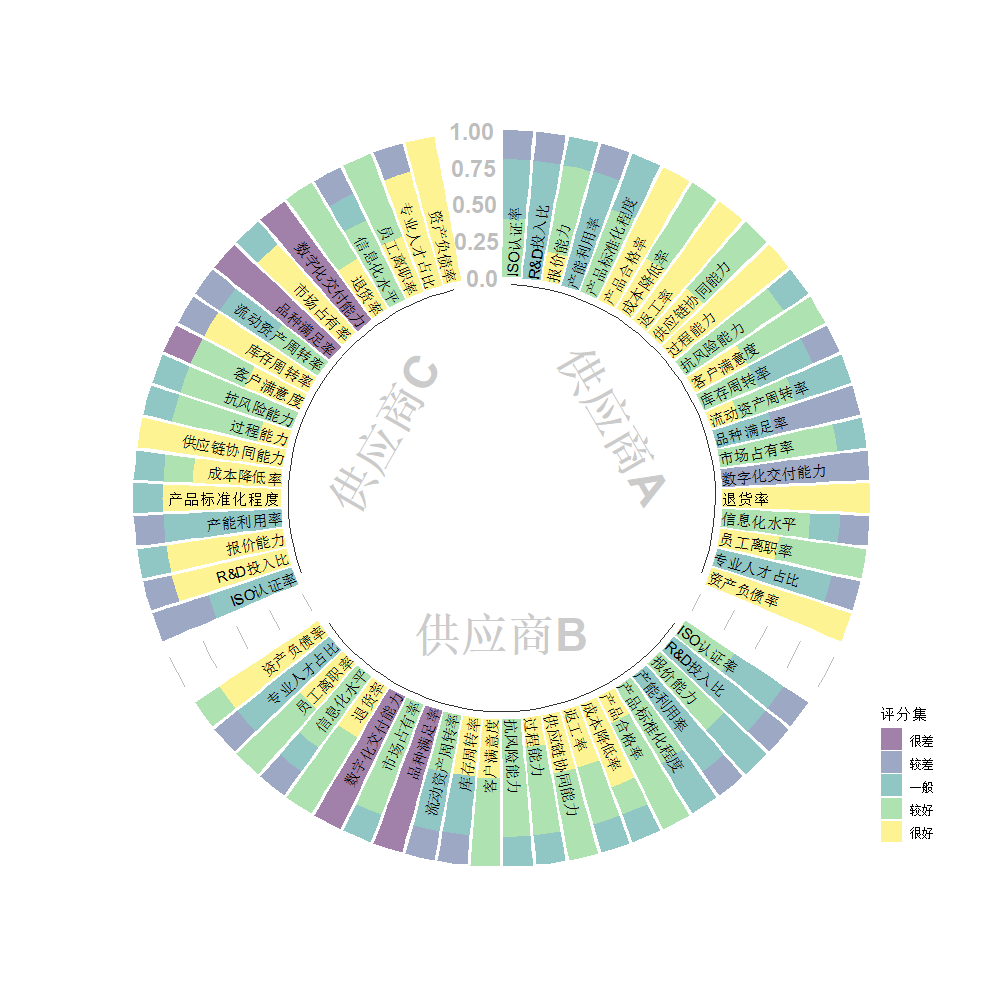
\includegraphics[height=0.8\textheight,trim=100 100 50 80,clip]{pic/supply.png}
		\caption{供应商评分图\footnote{邀请行业专家对以上三家供应商进行打
				分}}
		\label{supply}
	\end{figure}
\end{frame}

\begin{frame}{xxxxxxxxxxxxxxx}
	xxxxxxxxxxxxxxxxxxxxxxxxxxxxxxxxxxx
	
	\begin{minipage}{0.47\linewidth}	
		\scriptsize
		\begin{equation}
			R_{A1}=\left[ \begin{matrix}
				1 & 0 & 0 & 0 & 0 \\
				1 &  0 &  0  &  0  & 0 \\
				1 &  0  &  0 &  0  & 0 \\
				1 &  0  &  0  &  0  & 0 \\
			\end{matrix} \right] 
		\end{equation}	
	\end{minipage}
	\begin{minipage}{0.47\linewidth}
		\scriptsize
		\begin{equation}
			R_{A2}=\left[ \begin{matrix}
				1 &  0 &  0  &  0  & 0 \\
				0.4 &  0.6  &  0  &  0  & 0 \\ 
				0.2 &  0.6  &  0.2  &  0  & 0 \\ 
				0.2 &  0.4  &  0.4  &  0  & 0 \\ 
			\end{matrix} \right] 
		\end{equation}
	\end{minipage}

	\begin{minipage}{0.47\linewidth}
 \scriptsize
\begin{equation}
	R_{A3}=\left[ \begin{matrix}
		0 &  0  &  0  &  1  & 0 \\
		0 &  0  &  0.4  &  0.6  & 0 \\
		0 &  0  &  0.8  &  0.2  & 0 \\
		0 &  0.4  &  0.4  &  0.2  & 0 \\
	\end{matrix} \right] 
\end{equation}
	\end{minipage}	
	\begin{minipage}{0.47\linewidth}
 \scriptsize
\begin{equation}
	R_{A4}=\left[ \begin{matrix}
		0 &  0  &  0.8  &  0.2  & 0 \\
		0 &  0.4  &  0.4  &  0.2  & 0 \\
		0 &  0  &  0.8  &  0.2  & 0 \\
		0 & 0.6 & 0.4 & 0 & 0 \\
	\end{matrix} \right] 
\end{equation}
\end{minipage}


\begin{minipage}{0.47\linewidth}
 \scriptsize
\begin{equation}
	R_{A5}=\left[ \begin{matrix}
		0 & 0.6 & 0.2 & 0 & 0 \\
		0.4 &  0.6  &  0 &  0  & 0 \\
		0 &  0.8  &  0.2  &  0  & 0 \\
	\end{matrix} \right] 
\end{equation}
\end{minipage}	
\begin{minipage}{0.47\linewidth}
 \scriptsize
\begin{equation}
	R_{A6}=\left[ \begin{matrix}
		0 &  0.8  &  0.2  &  0  & 0 \\
		0.4 &  0.6  &  0 &  0  & 0 \\
		0.4 &  0.6  &  0 &  0  & 0 \\
	\end{matrix} \right] 
\end{equation}
\end{minipage}	

	\end{frame}

\begin{frame}{xxxxxxxxxxxxxxxx}
	xxxxxxxxxxxxxxxxxxxxxxxxxxxx
	
	\begin{equation}
			 \small
		\begin{aligned}
			P_{A1}&=B_1\times R_{A1}\\
			&=(0.4846,0.3031,0.1395,0.0705)\times \left[ \begin{matrix}
				1 & 0 & 0 & 0 & 0 \\
				1&  0  &  0  &  0  & 0 \\
				1 &  0  &  0 &  0  & 0 \\
				1&  0  &  0  &  0  & 0 \\
			\end{matrix} \right] \\
			&=(0.9977,0,0,0,0)^{T}\\
		\end{aligned}
	\end{equation}
\end{frame}

\begin{frame}{xxxxxxxxxxxxxxxxx}
	xxxxxxxxxxxxxxxxxxxxxxxxxxxxxx
	
	\begin{equation}
		\small
		R_{A}=
		\left[ \begin{matrix}
			P_{A1} \\
			P_{A2} \\
			P_{A3} \\
			P_{A4} \\
			P_{A5} \\
			P_{A6} \\
		\end{matrix} \right] 
		= \left[ \begin{matrix}
			0.99770&
			0.00000&
			0.00000&
			0.00000&
			0\\
			0.31350&
			0.52218&
			0.16432&
			0.00000&
			0\\
			0.00000&
			0.06896&
			0.34184&
			0.58910&
			0\\
			0.00000&
			0.36666&
			0.48172&
			0.15162&
			0\\
			0.12784&
			0.62440&
			0.13608&
			0.11168&
			0\\
			0.18416&
			0.70792&
			0.10792&
			0.00000&
			0\\
		\end{matrix} \right] 
	\end{equation}

xxxxxxxxxxxxxxxxxxxxxxxxxx
\end{frame}

\begin{frame}{xxxxxxxxxxxxxxxxxxxxx}
	xxxxxxxxxxxxxxxxxxxxxxxxxxxxxx
	
	\begin{equation}
			 \small
		\begin{aligned}
			S_A&=P_A\times U \\
			&=(0.45 ,0.23 ,0.15, 0.15 ,   0)\times (10,8,6,4,2)\\
			&=7.96\\
		\end{aligned}
	\end{equation}
	
	\begin{equation}
			 \small
		\begin{aligned}
			S_B&=P_B\times U \\
			&=(0.18 ,0.45 ,0.19, 0.04, 0.12)\times (10,8,6,4,2)\\
			&=7.07\\
		\end{aligned}
	\end{equation}
	
	\begin{equation}
			 \small
		\begin{aligned}
			S_C&=P_C\times U \\
			&=(0.33 ,0.28 ,0.15, 0.05, 0.16)\times (10,8,6,4,2)\\
			&=7.12\\
		\end{aligned}
	\end{equation}
	
\end{frame}	
	
\section{结论与展望}
\begin{frame}
	\qquad xxxxxxxxxxxxxxxxxxxxxxxxxxxxxxxx
	\vspace{5mm}
	\begin{itemize}
		\item xxxxxxxxxxxxxxxxxxxxxxxxxxx
		\item xxxxxxxxxxxxxxxxxxxxxxx\cite{1}
	\end{itemize}
\end{frame}	





\begin{frame}[allowframebreaks]
	\bibliographystyle{unsrt}
	\bibliography{ref}
\end{frame}

\begin{frame}
	\begin{center}
		{\Huge 请各位老师批评指正!}
	\end{center}
\end{frame}
\end{document}





